\documentclass[]{article}
\usepackage{lmodern}
\usepackage{amssymb,amsmath}
\usepackage{ifxetex,ifluatex}
\usepackage{fixltx2e} % provides \textsubscript
\ifnum 0\ifxetex 1\fi\ifluatex 1\fi=0 % if pdftex
  \usepackage[T1]{fontenc}
  \usepackage[utf8]{inputenc}
\else % if luatex or xelatex
  \ifxetex
    \usepackage{mathspec}
  \else
    \usepackage{fontspec}
  \fi
  \defaultfontfeatures{Ligatures=TeX,Scale=MatchLowercase}
\fi
% use upquote if available, for straight quotes in verbatim environments
\IfFileExists{upquote.sty}{\usepackage{upquote}}{}
% use microtype if available
\IfFileExists{microtype.sty}{%
\usepackage{microtype}
\UseMicrotypeSet[protrusion]{basicmath} % disable protrusion for tt fonts
}{}
\usepackage[margin=1in]{geometry}
\usepackage{hyperref}
\hypersetup{unicode=true,
            pdfborder={0 0 0},
            breaklinks=true}
\urlstyle{same}  % don't use monospace font for urls
\usepackage{natbib}
\bibliographystyle{apalike}
\usepackage{graphicx,grffile}
\makeatletter
\def\maxwidth{\ifdim\Gin@nat@width>\linewidth\linewidth\else\Gin@nat@width\fi}
\def\maxheight{\ifdim\Gin@nat@height>\textheight\textheight\else\Gin@nat@height\fi}
\makeatother
% Scale images if necessary, so that they will not overflow the page
% margins by default, and it is still possible to overwrite the defaults
% using explicit options in \includegraphics[width, height, ...]{}
\setkeys{Gin}{width=\maxwidth,height=\maxheight,keepaspectratio}
\IfFileExists{parskip.sty}{%
\usepackage{parskip}
}{% else
\setlength{\parindent}{0pt}
\setlength{\parskip}{6pt plus 2pt minus 1pt}
}
\setlength{\emergencystretch}{3em}  % prevent overfull lines
\providecommand{\tightlist}{%
  \setlength{\itemsep}{0pt}\setlength{\parskip}{0pt}}
\setcounter{secnumdepth}{0}
% Redefines (sub)paragraphs to behave more like sections
\ifx\paragraph\undefined\else
\let\oldparagraph\paragraph
\renewcommand{\paragraph}[1]{\oldparagraph{#1}\mbox{}}
\fi
\ifx\subparagraph\undefined\else
\let\oldsubparagraph\subparagraph
\renewcommand{\subparagraph}[1]{\oldsubparagraph{#1}\mbox{}}
\fi

%%% Use protect on footnotes to avoid problems with footnotes in titles
\let\rmarkdownfootnote\footnote%
\def\footnote{\protect\rmarkdownfootnote}

%%% Change title format to be more compact
\usepackage{titling}

% Create subtitle command for use in maketitle
\providecommand{\subtitle}[1]{
  \posttitle{
    \begin{center}\large#1\end{center}
    }
}

\setlength{\droptitle}{-2em}

  \title{}
    \pretitle{\vspace{\droptitle}}
  \posttitle{}
    \author{}
    \preauthor{}\postauthor{}
    \date{}
    \predate{}\postdate{}
  
\usepackage{booktabs}
\usepackage{longtable}
\usepackage{array}
\usepackage{multirow}
\usepackage{wrapfig}
\usepackage{float}
\usepackage{colortbl}
\usepackage{pdflscape}
\usepackage{tabu}
\usepackage{threeparttable}
\usepackage{threeparttablex}
\usepackage[normalem]{ulem}
\usepackage{makecell}
\usepackage{xcolor}

\usepackage{float} \usepackage{caption} \captionsetup[table]{font=footnotesize} \captionsetup[figure]{font=footnotesize} \usepackage{setspace}\onehalfspacing \usepackage{lineno}\linenumbers

\begin{document}

\textbf{Title:} Global patterns of forest autotrophic carbon fluxes

\textbf{Running head:}

\textbf{Authors:}

Rebecca Banbury Morgan\textsuperscript{1,2}

Valentine Herrmann\textsuperscript{1}

Norbert Kunert\textsuperscript{1,3}

Ben Bond-Lamberty\textsuperscript{4}

Helene C. Muller-Landau\textsuperscript{3}

Kristina J. Anderson-Teixeira\textsuperscript{1,3}*

\textbf{Author Affiliations:}

\begin{enumerate}
\def\labelenumi{\arabic{enumi}.}
\item
  Conservation Ecology Center; Smithsonian Conservation Biology
  Institute; National Zoological Park, Front Royal, VA, USA
\item
  \emph{Becky- current}
\item
  Center for Tropical Forest Science-Forest Global Earth Observatory;
  Smithsonian Tropical Research Institute; Panama, Republic of Panama
\item
  Joint Global Change Research Institute, Pacific Northwest National
  Laboratory, College Park Maryland 20740 USA
\end{enumerate}

*Corresponding Author:

phone: 1-540-635-6546

fax:1-540-635-6506

email: \href{mailto:teixeirak@si.edu}{\nolinkurl{teixeirak@si.edu}}

\textbf{Keywords:}

\textbf{Paper type:} Primary Research Article

\newpage

\subsubsection{Abstract}\label{abstract}

{[}\textbf{very rough start:}{]} Carbon fixation, allocation, and
metabolism by trees set the basis for energy and material flows in
forest ecosystems and define their interactions with Earth's changing
climate. Here, we drew upon \# records from the Global Forest Carbon
Database (ForC), representing all major forest types and the nine most
significant forest autotrophic carbon flux (FACF) variables, to
comprehensively explore how C cycling in mature, undisturbed forests
varies with latitude and climate on a global scale. We show that, across
all FACF variables analyzed, C cycling decreases linearly with latitude
-- a finding that confirms multiple previous studies but contradicts the
idea that net primary productivity (\(NPP\)) of temperate forests rivals
that of tropical forests. The FACF variables generally increase in
proportion to one another, with few differences in allocation detectable
at this global scale, but differed in that latitude explained a lower
proportion of variation among subsidiary fluxes (in particular, woody
aboveground \(NPP\) and belowground \(NPP\), \(BNPP\)). Climate
explained a significant proportion (\#-\#\%) of variation in all C
fluxes analyzed (less for subsidiary fluxes), with temperature variables
in general and mean annual temperature (\(MAT\)) in particular being the
best predictors of FACF on this global scale. While other climate
variables (\emph{e.g.}, \textbf{XX}) displayed significant correlation
with FACF, none of them had significantly better explanatory power than
\(MAT\). The effects of temperature were modified by moisture
availability, with reduced FACF under hot and dry conditions and
sometimes under very high precipitaiton (especially for \(BNPP\)). FACF
declined with temperature seasonality, but growing season length doesn't
improve upon MAT as a predictor. Within the growing season, the
influence of climate on C cycling is smaller but still significant for a
number of carbon fluxes. These findings clarify the big picture of how
FACF varies with latitude and climate on a global scale. As we enter a
period of accelerating climatic change, understanding of the fundamental
climatic controls on FACF sets a foundation for understanding patterns
of change.

\newpage

\subsubsection{Introduction}\label{introduction}

Carbon cycling in forests worldwide provides the energetic basis for
sustaining the majority of Earth's terrestrial biodiversity and many
human populations (\textbf{REF}), while strongly influencing atmospheric
CO\textsubscript{2} and climate \citep{bonan_forests_2008}. Forests'
autotrophic carbon fluxes (FACF)--that is, carbon fixation, allocation,
and metabolism by trees and other primary producers--sets the energy
ultimately available to heterotrophic organisms (including microbes), in
turn influencing their abundance (\textbf{REFS}) and possibly diversity
\citep{waide_relationship_1999} (\textbf{REFS}). FACF influences all
organic matter stocks in forest ecosystems and is linked to cycling of
energy, water, and nutrients (\textbf{REFS}) \citep{piao_forest_2010}.
Critically, FACF also define forest interactions with Earth's changing
climate. Over 69 Gt of CO\textsubscript{2} cycle through Earth's forests
each year \citep{badgley_terrestrial_2019}, and in recent decades their
net C sequestration (\textasciitilde{}2.4 Gt C yr\textsuperscript{-1})
offset roughly 30\% of anthropogenic fossil fuel emissions
\citep{pan_large_2011}. As atmospheric carbon dioxide levels continue to
rise, driving climate change, forests will play a critical role in
shaping the future of Earth's climate
\citep{cavaleri_urgent_2015, rogelj_mitigation_2018}. However, our
ability to draw general macroscopic conclusions regarding global
variation in FACF with respect to climate has been limited in that these
analyses often mix forests that vary in stand age, disturbance history,
and/or management status; do not always sufficiently parse related
variables; and typically consider only one or a few variables at a time.

FACF decrease with latitude, but it remains unclear whether and how the
shape of this relationship varies across fluxes. Studies agree that FACF
are lowest in the boreal regions, and increase into the temperate
regions
\citep{luyssaert_co_2007, huston_global_2009, beer_terrestrial_2010, jung_global_2011}.
However, evidence is inconclusive on whether primary productivity
continues to increase into the tropics, or whether it plateaus in
temperate regions. Evidence for this is further complicated by the fact
that different studies use different measures of productivity to explore
these relationships. For example, modelling of global terrestrial
ecosystem gross primary productivity (\(GPP\)) through upscaling and
calibration of eddy flux measurements indicates that GPP peaks in
tropical forests
\citep{beer_terrestrial_2010, jung_global_2011, badgley_terrestrial_2019, li_mapping_2019}.
In contrast, some studies suggest that the highest values of net primary
productivity (\(NPP\)) may be found in temperate forests
\citep{luyssaert_co_2007, huston_global_2009}, while others find \(NPP\)
highest in the tropics and decreasing with latitude
\citep{simova_enigma_2017}. Other studies have chosen to focus
exclusively on above-ground net primary productivity (\(ANPP\)), finding
evidence of a weak negative relationship between \(ANPP\) and latitude
\citep{huston_global_2009, gillman_latitude_2015}.

The latitudinal gradient in FACF is primarily driven by climate, which
is a significant driver of FACF across broad spatial scales
\citep{luyssaert_co_2007, cleveland_relationships_2011, hursh_sensitivity_2017}.
The majority of studies have focused on exploring the relationships of
FACF to mean annual temperature (MAT) and mean annual precipitation
(MAP), as the most commonly reported site-level climate variables. While
these fail to capture some important aspects of climate such as
seasonality, they do describe broad trends in temperature and water
availability, and therefore capture a substantial portion of
global-scale variation in climate. There is strong evidence that both
MAT and MAP show significant positive relationships with FACF
\citep{chu_does_2016}. However, as with latitude, the shape of those
relationships is not always clear, and, again, is complicated by the use
of different measures of FACF across studies. Various measures of
primary productivity \{\textbf{FACF?}\} saturate at high levels of MAP,
though the saturation points identified vary from 1500mm
\citep{luyssaert_co_2007} up to 2445mm MAP
\citep{schuur_productivity_2003}. Studies of the influence of MAT on
productivity \{\textbf{FACF?}\} are less conclusive. Luyssaert et al.
\citeyearpar{luyssaert_co_2007} examined GPP and NPP and found that,
while \(GPP\) increases linearly with MAT, NPP saturates at around
10\(^\circ\)C MAT. In contrast, Larjavaara and Muller-Landau
\citeyearpar{larjavaara_temperature_2012}, find that increases in
\(GPP\) saturate at approximately 25\(^\circ\)C MAT, while Schuur
\citeyearpar{schuur_productivity_2003} shows that \(NPP\) increases
linearly with temperature. Taylor et al.
\citeyearpar{taylor_temperature_2017} showed a positive interaction
between MAT and MAP in shaping tropical forest productivity, such that
high rainfall had a negative effect on productivity in cooler climates,
compared to a positive effect in warmer climates. \{\textbf{It would be
good to add some more citations on soil respiraiton. I'm sure BBL can
help.}\}

FACF can be influenced by many other factors as well, which often act
across a range of scales, and may show interactive effects with each
other \citep{cleveland_relationships_2011}. On a local scale, stand age
\citep{litton_carbon_2007, gillman_latitude_2015}, biodiversity
\citep{liang_positive_2016}, management \citep{simova_enigma_2017},
nutrient availability \citep{aragao_above_2009}, and altitude
\citep{girardin_net_2010, malhi_variation_2017} all impact FACF. On a
global scale, we expect that FACF are most strongly influenced by broad
climatic gradients. There is evidence that FACFs also respond to
variables such as cloud cover \citep{taylor_temperature_2017}, solar
radiation \citep{fyllas_solar_2017}, and potential evapotranspiration
\citep{kerkhoff_plant_2005} in potentially significant ways.
Furthermore, MAT and MAP are very coarse measures of climate, and so
fail to capture much variation in climate on an intra-annual scale,
including the effects of factors such as growing season length, number
of frost-free days, temperature seasonality, and dry season length. Some
studies have suggested that the apparently strong relationship between
MAT and FACFs is actually a consequence of the correlation between MAT
and growing season length
\citep{kerkhoff_plant_2005, malhi_productivity_2012, michaletz_convergence_2014, michaletz_drivers_2018}.
Kerkhoff et al. \citeyearpar{kerkhoff_plant_2005} and Michaletz et al.
\citeyearpar{michaletz_convergence_2014} find that, within the growing
season, there is no significant relationship between primary
productivity and MAT, suggesting that the effect of temperature is due
to increased length of growing season, rather than an inherent influence
of temperature on FACF.

The recent development of the Global Forest Carbon database (ForC),
which synthesizes multiple variables and including records of stand
history
\citep{anderson-teixeira_carbon_2016, anderson-teixeira_forc_2018},
opens up the possibility for a standardized analysis of global scale
variation in multiple FACF and the principle climatic drivers of these
patterns. In order to approach this broad topic, we simplify the major
gaps in our knowledge to five broad questions and corresponding
hypotheses (Table 1). First, we ask how FACF vary with latitude. We then
test how these fluxes relate to MAT and MAP, and additionally how they
respond to other, less well-studied, climate variables. Finally, we
consider the relationship between FACF and seasonality, considering the
role of seasonality in explaining variation in carbon fluxes, and the
influence of climate on FACF standardized by growing season length. We
address the above questions for nine carbon fluxes contained in ForC,
allowing for an in-depth exploration of the effect of climate on FACF
globally.

\renewcommand{\arraystretch}{2}

\begin{landscape}\begin{table}[!h]

\caption{\label{tab:unnamed-chunk-4}Summary of research questions, corresponding hypotheses, and results. Statistically signficant support for/ rejection of hypotheses is indicated with 'yes'/'no', parentheses indicate partial overall support/rejection of hypotheses across all FACF, and '-' indicates no significant relationship.}
\centering
\resizebox{\linewidth}{!}{
\fontsize{12}{14}\selectfont
\begin{tabular}{llllllllllll}
\toprule
\multicolumn{1}{c}{ } & \multicolumn{1}{c}{ } & \multicolumn{9}{c}{Forest autotrophic carbon fluxes (FACF)} & \multicolumn{1}{c}{ } \\
\cmidrule(l{3pt}r{3pt}){3-11}
Questions and hypotheses (with related references) & Overall & $GPP$ & $NPP$ & $ANPP$ & $ANPP_{woody.stem}$ & $ANPP_{foliage}$ & $BNPP$ & $BNPP_{fine.root}$ & $R_{auto}$ & $R_{auto-root}$ & Support\\
\midrule
\addlinespace[1em]
\multicolumn{5}{l}{\textbf{Q1. How do FACF vary with latitude?}}\\
\hspace{1em}H1.1. FACF decrease linearly with latitude.\textsuperscript{1}$^{,}$\textsuperscript{2}$^{,}$\textsuperscript{3} & yes & yes & yes & yes & yes & yes & yes & yes & yes & yes & Fig. 2\\
\addlinespace[1em]
\hline
\multicolumn{5}{l}{\textbf{Q2. How do FACF vary with MAT and MAP?}}\\
\hspace{1em}H2.1. FACF increase with MAT.\textsuperscript{1}$^{,}$\textsuperscript{4} & yes & yes & yes & yes & yes & yes & yes & yes & yes & yes & Figs. 4, S4, S5\\
\hspace{1em}H2.2. FACF increase with precipitation.\textsuperscript{1}$^{,}$\textsuperscript{4} & (yes) & yes & yes & yes & - & yes & yes & yes & yes & yes & Figs. 4, S4, S5\\
\hspace{1em}H2.3. Temperature and precipitation interactively shape FACF.\textsuperscript{5} & (yes) & yes & yes & - & yes & - & yes & yes & yes & - & Fig. 3\\
\addlinespace[1em]
\hline
\multicolumn{5}{l}{\textbf{Q3. How are FACF related to other climate variables?}}\\
\hspace{1em}H3.1. FACF increase with PET. & yes & yes & yes & yes & yes & yes & yes & yes & yes & yes & Figs. 4, S4, S5\\
\hspace{1em}H3.2. FACF increase with vapour pressure deficit. & yes & yes & yes & yes & yes & yes & yes & yes & yes & yes & Figs. 4, S4, S5\\
\hspace{1em}H3.3. FACF increase with solar radiation. & (yes) & yes & yes & yes & yes & yes & yes & yes & yes & - & Figs. S4, S5\\
\addlinespace[1em]
\hline
\multicolumn{5}{l}{\textbf{Q4. How does seasonality influence FACF?}}\\
\hspace{1em}H4.1. FACF decrease with temperature seasonality. & yes & yes & yes & yes & yes & yes & yes & yes & yes & yes & Figs. 4, S6, S7\\
\hspace{1em}H4.2. FACF decrease with precipitation seasonality. & - & - & - & - & - & - & - & - & - & - & Figs. S6, S7\\
\hspace{1em}H4.3. FACF increase with growing season length.\textsuperscript{6}$^{,}$\textsuperscript{7}$^{,}$\textsuperscript{8} & yes & yes & yes & yes & yes & yes & yes & yes & yes & yes & Figs. 4, S6, S7\\
\hspace{1em}H4.4. Growing season length is a better predictor of FACF than MAT.\textsuperscript{7}$^{,}$\textsuperscript{8} & (no) & no & no & no & no & no & no & - & no & no & Table S4\\
\addlinespace[1em]
\hline
\multicolumn{5}{l}{\textbf{Q5. When standardised by growing season length, how do FACF vary with climate?}}\\
\hspace{1em}H5.1. Growing season FACF increase with temperature.\textsuperscript{8} & (yes) & - & - & yes & - & yes & - & - & - & - & Figs. S8, S9\\
\hspace{1em}H5.2. Growing season FACF increase with PET. & (yes) & yes & yes & - & yes & - & yes & yes & - & - & Figs. S8, S9\\
\hspace{1em}H5.3. Growing season FACF increase with precipitation. & (yes) & - & - & yes & - & yes & - & - & - & - & Figs. S8, S9\\
\hspace{1em}H5.4. Growing season FACF increase with solar radiation. & (yes) & yes & yes & - & - & - & yes & yes & - & - & Figs. S8, S9\\
\bottomrule
\multicolumn{12}{l}{\textsuperscript{1} Luyssaert et al. (2007) \textsuperscript{2} Gillman et al. (2015) \textsuperscript{3} Simova and Storch (2017) \textsuperscript{4} Schuur (2003) \textsuperscript{5} Taylor et al. (2016) \textsuperscript{6} Malhi (2012) \textsuperscript{7} Michaletz et al. (2014) \textsuperscript{8} Chu et al. (2016)}\\
\end{tabular}}
\end{table}
\end{landscape}

\subsubsection{Materials and Methods}\label{materials-and-methods}

\emph{Forest carbon flux data}

This analysis focused on nine FACF included in the open-access ForC
database (Table 2)
\citep{anderson-teixeira_carbon_2016, anderson-teixeira_forc_2018}. ForC
contains records of field-based measurements of forest carbon stocks and
annual fluxes, compiled from original publications and existing data
compilations and databases. Associated data, such as stand age,
measurement methodologies, and disturbance history, are also included.
The database was significantly expanded since the publication of
\citet{anderson-teixeira_forc_2018} through integration with the Global
Soil Respiration Database \citep{bond-lamberty_global_2010}. Additional
targeted literature searches were conducted to identify any further
available data on the FACF analyzed here, with particular focus on
mature forests in temperate and boreal regions, which were not included
in the review of \citet{anderson-teixeira_carbon_2016}. We used ForC
v3.0, archived on Zenodo with DOI 10.5281/zenodo.3403855. This version
contained 29,730 records from 4,979 plots, representing 20 distinct
ecozones across all forested biogeographic and climate zones.

This analysis focused on mature forests with no known history of
signficant disturbance or management. There is evidence that stand age
influences patterns of FACF and carbon allocation in forest ecosystems,
and can confound relationships between latitude and primary productivity
\citep{delucia_forest_2007, gillman_latitude_2015}. To reduce any
biasing effects of stand age, we included only stands of known age
\(\ge\) 100 years and those described by terms such as ``mature'',
``intact'', or ``old-growth''. Since management can alter observed
patterns of FACF \citep{simova_enigma_2017}, sites were excluded from
analysis if they were managed, defined as plots that were planted,
managed as plantations, irrigated, fertilised or including the term
``managed'' in their site description. Sites that had experienced
significant disturbance within the past 100 years were also excluded.
Disturbances that qualified sites for exclusion included major cutting
or harvesting, burning, flooding, drought and storm events with site
mortality \textgreater{}10\% of trees. Grazed sites were retained.

\begin{table}[!h]

\caption{\label{tab:unnamed-chunk-5}Definitions and sample sizes of FACF variables used in analysis. All variables are in units of Mg C ha$^{-1}$ yr$^{-1}$. }
\centering
\resizebox{\linewidth}{!}{
\fontsize{12}{14}\selectfont
\begin{tabular}{l>{\raggedright\arraybackslash}p{4cm}>{\raggedright\arraybackslash}p{7cm}>{\raggedright\arraybackslash}p{10cm}>{\raggedleft\arraybackslash}p{1.5cm}>{\raggedleft\arraybackslash}p{1.5cm}}
\toprule
\multicolumn{1}{c}{ } & \multicolumn{1}{c}{ } & \multicolumn{1}{c}{ } & \multicolumn{1}{c}{ } & \multicolumn{2}{c}{Sample size} \\
\cmidrule(l{3pt}r{3pt}){5-6}
Variable & Definition & Components included & Methodologies & records & geographic areas\textsuperscript{*}\\
\midrule
$GPP$ & Gross Primary Production & full ecosystem & flux partitioning of eddy-covariance; $NPP$+$R_{auto}$ & 243 & 49\\
$NPP$ & Net Primary Production & stem, foliage, coarse root, fine root, optionally others (e.g., branch, reproductive, understory) & $ANPP$ + $BNPP$ (majority); $GPP$-$R_{auto}$ & 161 & 56\\
$ANPP$ & Aboveground $NPP$ & stem, foliage, optionally others (e.g., branch, reproductive, understory) & $ANPP_{woody-stem}$ + $ANPP_{foliage}$ (+ others) & 278 & 86\\
$ANPP_{woody.stem}$ & Woody stem growth component of $ANPP$ & woody stems down to DBH $\le$ 10cm (no branch turnover) & stem growth measurements scaled to biomass using allometries & 264 & 96\\
$ANPP_{foliage}$ & Foliage component of $ANPP$ & foliage & litterfall collection (separated into components) & 98 & 49\\
\addlinespace
$BNPP$ & Belowground $NPP$ & coarse and fine roots & coarse roots estimated indirectly using allometries based on aboveground stem increment measures ; fine roots as below & 101 & 48\\
$BNPP_{fine.root}$ & Fine root component of $BNPP$ & fine roots & measurements combined one or more of the following: soil cores, minirhizotrons, turnover estimates,  root ingrowth cores & 88 & 41\\
$R_{auto}$ & Autotrophic respiration & foliage, stem, and root & chamber measurements of foliage and stem gas exchange +  $R_{auto-root}$ (as below) & 22 & 13\\
$R_{auto-root}$ & Root respiration & (coarse and) fine roots & partitioning of total soil respiration (e.g., through root exclusion), scaling of root gas exchange; excluded alkali absoption and soda lime methods for measuring soil respiration & 64 & 26\\
\bottomrule
\multicolumn{6}{l}{\textsuperscript{*} Geographic areas group geographically proximate sites, defined using a hierarchical cluster analysis on the distance matrix of the sites, and a cutoff of 25km}\\
\end{tabular}}
\end{table}

\begin{figure}[H]
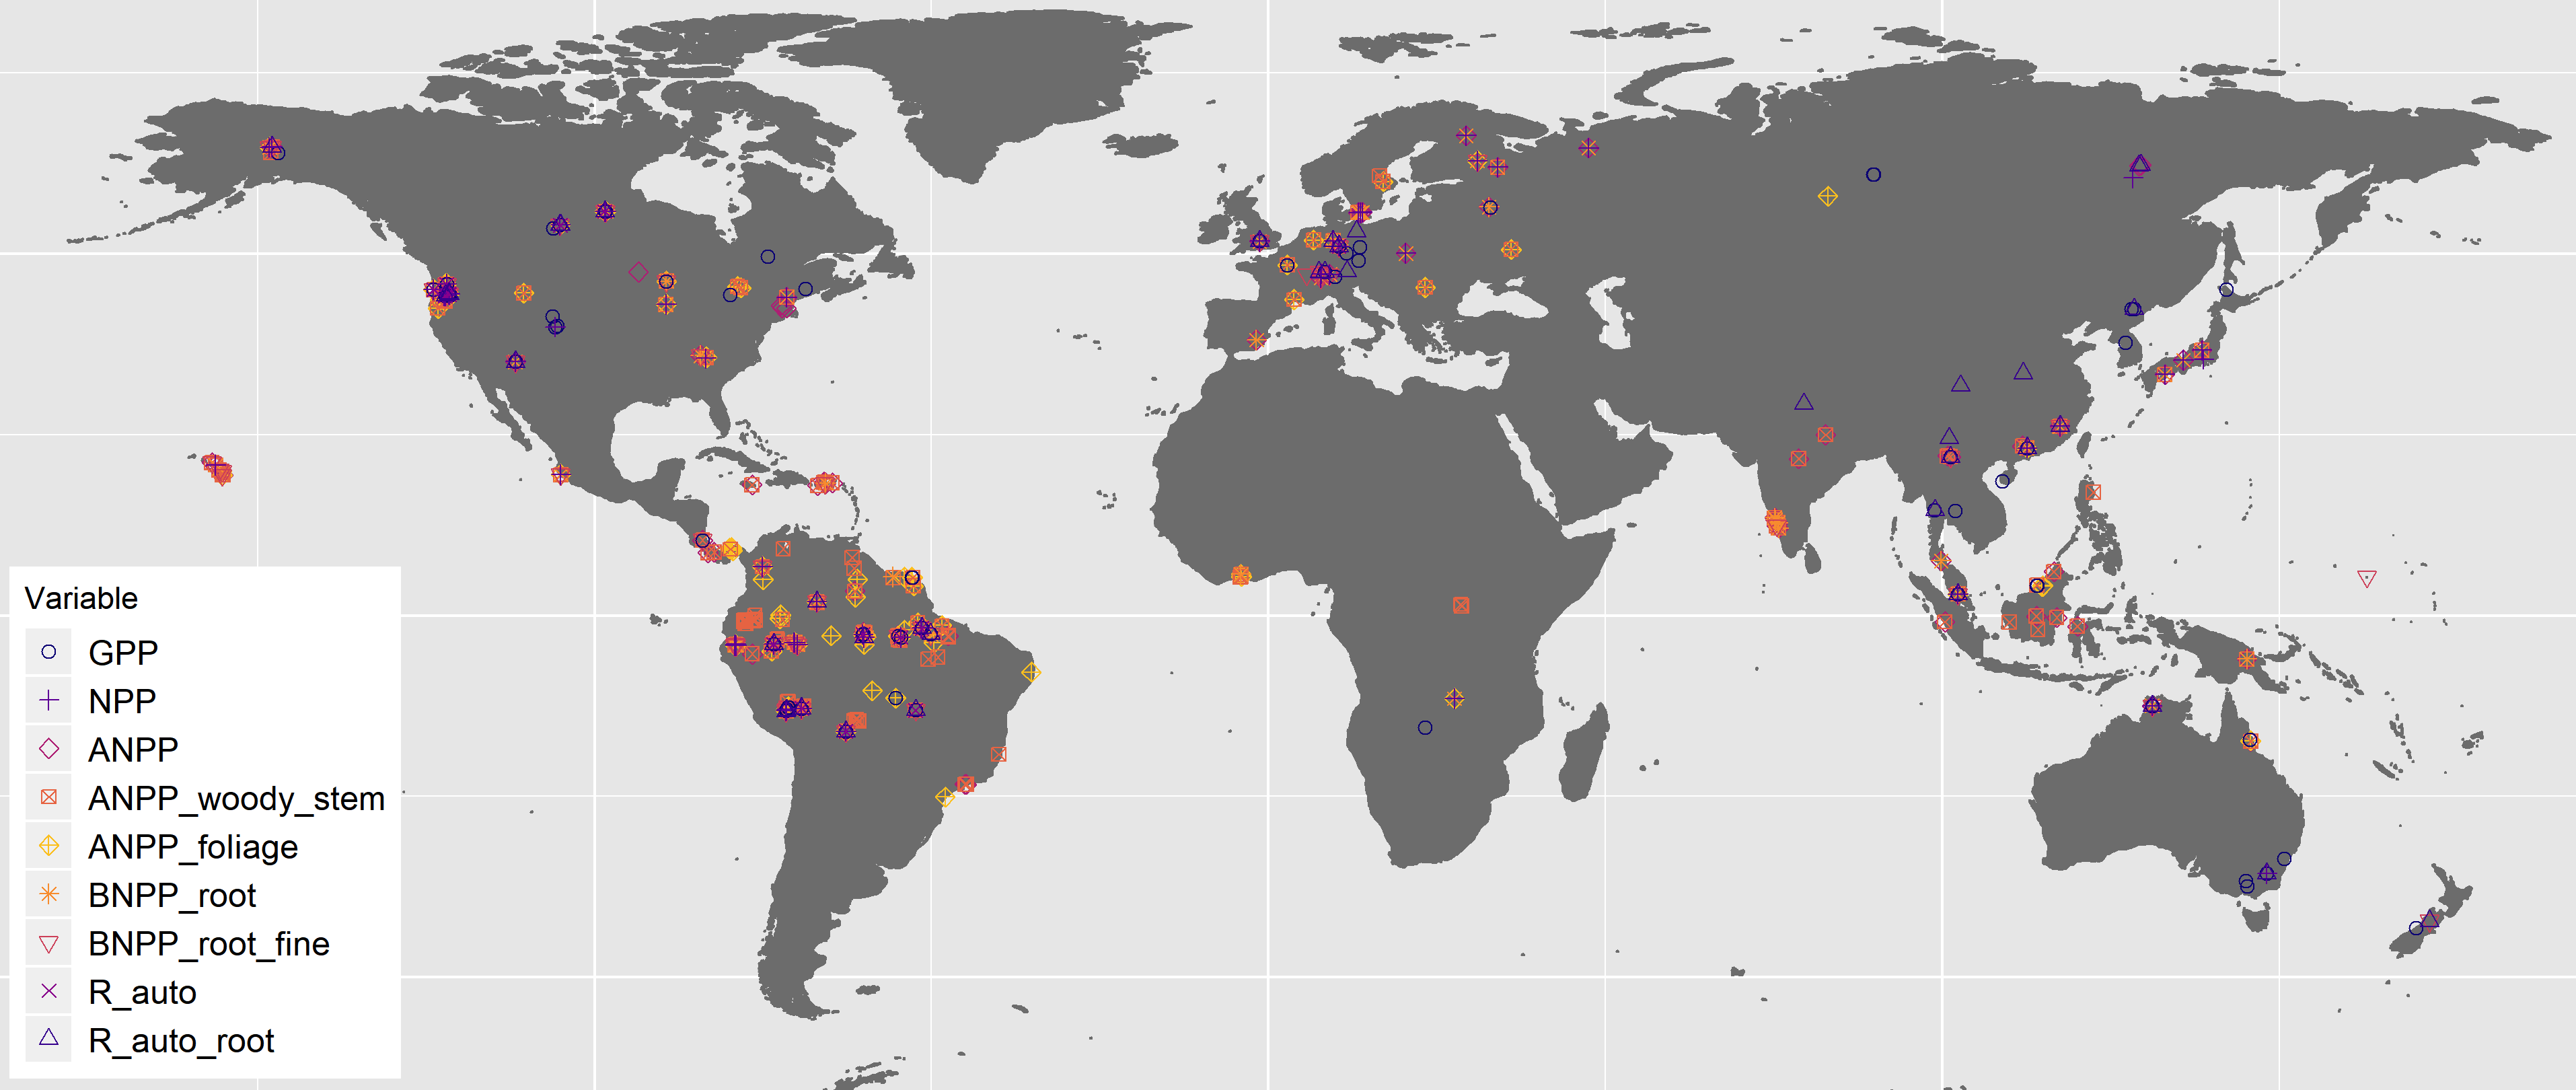
\includegraphics[width=1\linewidth]{distribution_all_variables_cropped} \caption{Map showing all data used in the analysis, coded by variable. Variables are plotted individually in Fig. S1. }\label{fig:unnamed-chunk-6}
\end{figure}

\emph{Climate data}

ForC contains geographic coordinates associated with each measurement
record and, when available, mean annual temperature (MAT) and mean
annual precipitation (MAP) as reported in the primary literature
\citep{anderson-teixeira_forc_2018}. Based on the geographic
co-ordinates for each site, data on twelve climate variables--including
MAT, MAP, temperature and precipitation seasonality, annual temperature
range, solar radiation, cloud cover, annual frost and wet days,
potential evapotranspiration (PET), aridity (MAP/PET), and vapor
pressure deficit (VPD)--were extracted from five open-access climate
datasets: WorldClim \citep{hijmans_very_2005}, WorldClim2
\citep{fick_worldclim_2017}, the Climate Research Unit (CRU) time-series
dataset v. 4.03 \citep{harris_updated_2014}, the Global Aridity Index
and Potential Evapotranspiration Climate Database
\citep{trabucco_global_2019}, and TerraClimate
\citep{abatzoglou_terraclimate_2018} (Table S1). From these data, we
derived maximum VPD, defined as the VPD of the month with the largest
deficit, and the number of water stress months, defined as the number of
months annually where precipitation was lower than PET. Where site-level
data was missing for MAT or MAP, we used values from the WorldClim
dataset.

Length of the growing season was estimated to the nearest month, where
growing season months were defined as months with mean minimum
temperature \textgreater{} 0.5\(^\circ\)C. We experimented with a
definion of growing season months including a moisture index, defined as
(MAT - PET)/PET, \textgreater{} -0.95 (Kerkhoff et al. 2005; see also
Michaletz et al. 2014). However, we found that including a moisture
index had \textbf{no} effect on the estimates of growing season length,
and so chose to exclude it. (\textbf{Becky, was it really no effect? or
minimal?}) Monthly data for PET, precipitation, and temperature from the
CRU dataset v 4.03 \citep{harris_updated_2014}, and solar radiation from
WorldClim2 \citep{fick_worldclim_2017} were used to calculate mean
monthly PET, precipitation, temperature and solar radiation during the
growing season. Total growing season precipitation and solar radiation
were also calculated.

\emph{Analyses}

The effects of latitude and climate on FACF were analysed using mixed
effects models using the package `lme4' \citep{bates_fitting_2015} in R
v.3.5.1 \citep{r_core_team_r:_2018}. The basic model for all analyses
included a fixed effect of latitude or climate and a random effect of
plot nested within geographic area. Geographic areas--\emph{i.e.},
spatially clustered sites--are defined within ForC using a hierarchical
cluster analysis on the distance matrix of the sites and a cutoff of
25km \citep{anderson-teixeira_forc_2018}. We experimented with inclusion
of altitude as a fixed effect, but excluded it from the final models
because it added very little explanatory power--that is, the difference
in AIC (\(\Delta\)AIC) relative to models excluding altitude was
generally small (often \(\Delta\)AIC\textless{}2). Hypotheses were
accepted if the \(\Delta\)AIC between a model including the fixed effect
of interest and a corresponding null model excluding that fixed effect
exceeded 2.0. All \(R^2\) values presented here are marginal \(R^2\)
values, and refer to the proportion of variation explained by only the
fixed effects. Specific analyses are as described below.

We first examined the relationship between latitude and FACF (Q1; Table
1). We tested models with latitude as a linear term (corresponding null:
model without latitude) and as a second-order polynomial term
(corresponding null: model with latitude as a linear term), and
calculated AIC values to determine the best model. Models were accepted
as the best model if \(\Delta\)AIC \textgreater{} 2 with respect to the
corresponding null, and were significant with respect to a null model
with no fixed term. We also examined relationships among fluxes across
latitude, testing whether sums of component fluxes matched the larger
fluxes and whether C allocation varied with latitude, as specified
below.

To test whether trends in component fluxes across latitude sum to match
those of larger fluxes, regression lines for smaller component fluxes
were summed to generate new estimates of larger fluxes, which were then
compared against the latitudinal regression of the larger flux.
Confidence intervals for the larger flux were calculated using the
`bootMer' function from the lme4 package \citep{bates_fitting_2015}.
This analysis was applied to following sets of fluxes: (1)
\(GPP = NPP + R_{auto}\), (2) \(NPP = ANPP + BNPP\), and (3)
\(ANPP = ANPP_{foliage} + ANPP_{woody.stem}\). In addition, we estimated
total belowground C flux (TBCF, not analyzed due to limited data) as
\(TBCF = BNPP + R_{root}\).

Variation in allocation to component carbon fluxes along latitudinal
gradients was explored for the following pairings: \(GPP:NPP\),
\(ANPP:BNPP\), \(ANPP_{foliage}:ANPP_{woody.stem}\),
\(ANPP_{foliage}:NPP\), \(ANPP_{woody.stem}:NPP\), \(ANPP:NPP\), and
\(BNPP:NPP\). For each set of paired fluxes, measurements taken at the
same site and plot, and in the same year, were paired together, and the
ratio of each pair of measurements calculated. The ratios were regressed
against latitude and climate variables, using the linear model specified
above. Cook's distance analyses were carried out for each of the models,
and indicated that data from a few high-elevation sites were having a
disproportionate influence on the regressions. To account for this,
models were re-run using only data from sites \(\le\) 1000m.

We next examined the relationships of FACF to climate variables (Q2-Q4;
Table 1). As with latitude, we tested both linear and polynomial fits
for each climate variable. We tested relationships of each FACF (Table
2) against each climate variable (Table S1), but focus
presentation--including focal hypotheses (Table 1)--on climate variables
that explained \textgreater{}20\% of variation in FACF. \textbf{Becky,
please make this more specific. I drafted this based on the results, but
its not very clear.}

To investigate the potential joint and interactive effects of climate
variables on carbon fluxes, multivariate models were also specified. We
explored a large range of climate variable combinations and ultimately
decided to focus on MAT and MAP. We favored these over variables with
similar explanatory power because they are the most commonly reported
climate variables and are recorded in ForC. MAT was consistently among
the best individual predictors of FACF (Table S2), although it was
occasionally out-performed by closely correlated climate variables (Fig.
S2). In combination with MAT as a primary climate variable, MAP was
consistently among the best secondary climate variables. Specifically,
compared again a model including MAT x MAP, there were no other
variables that, in interaction with MAT, improved AIC by
\textgreater{}2.0 and \(R^2\) by \textgreater{}0.05. In examinging the
joint and interactive effects of climate variables, an additive model
including MAT and MAP as fixed effects was accepted when \(\Delta\)AIC
\textgreater{}2 relative to a null including only MAT as a fixed effect.
An interactive model including an MAT x MAP interaction was accepted
when \(\Delta\)AIC \textgreater{}2 relative to a null including MAT and
MAP as fixed effects.

To test whether and how FACF varied with climate when standardised by
growing season length (Q5), we first standardized FACF by dividing by
growing season length (as defined above). We then tested for
correlations between growing season length-standardised FACF against
growing season climate variables. For analyses on data within the
growing season, only linear models were specified.

\textbf{All analyses were conducted in R (}Version\textbf{). Code and
results are archived on GitHub\ldots{}.}

\subsubsection{Results}\label{results}

In total, we analyzed 1228 records from nine FACF variables taken from
forests that had experienced no major anthropogenic disturbances within
the past 100 years. These records represented a total of 154 distinct
geographic areas across all forested biogeographic and climate zones
(Fig. 1, Table 2).

\emph{How do FACF vary with latitude?}

All major carbon fluxes decreased linearly with latitude (Fig. 2; Table
S2). Latitude was a strong predictor for many of the carbon
fluxes--particularly the larger fluxes (Table S2). Specifically,
latitude explained 64\% of variation in GPP (n = 254,
p\textless{}0.0001), 50\% in NPP (n = 114, p\textless{}0.0001) and 45\%
in ANPP (n = 259, p\textless{}0.0001). The FACF that were most poorly
predicted by latitude were \(BNPP_{root-fine}\) (\(R^2\)=0.17) and
\(ANPP_{woody.stem}\) (\(R^2\)=0.18). For all FACF, the relationship
with latitude was best predicted by the linear model).

\begin{figure}[H]
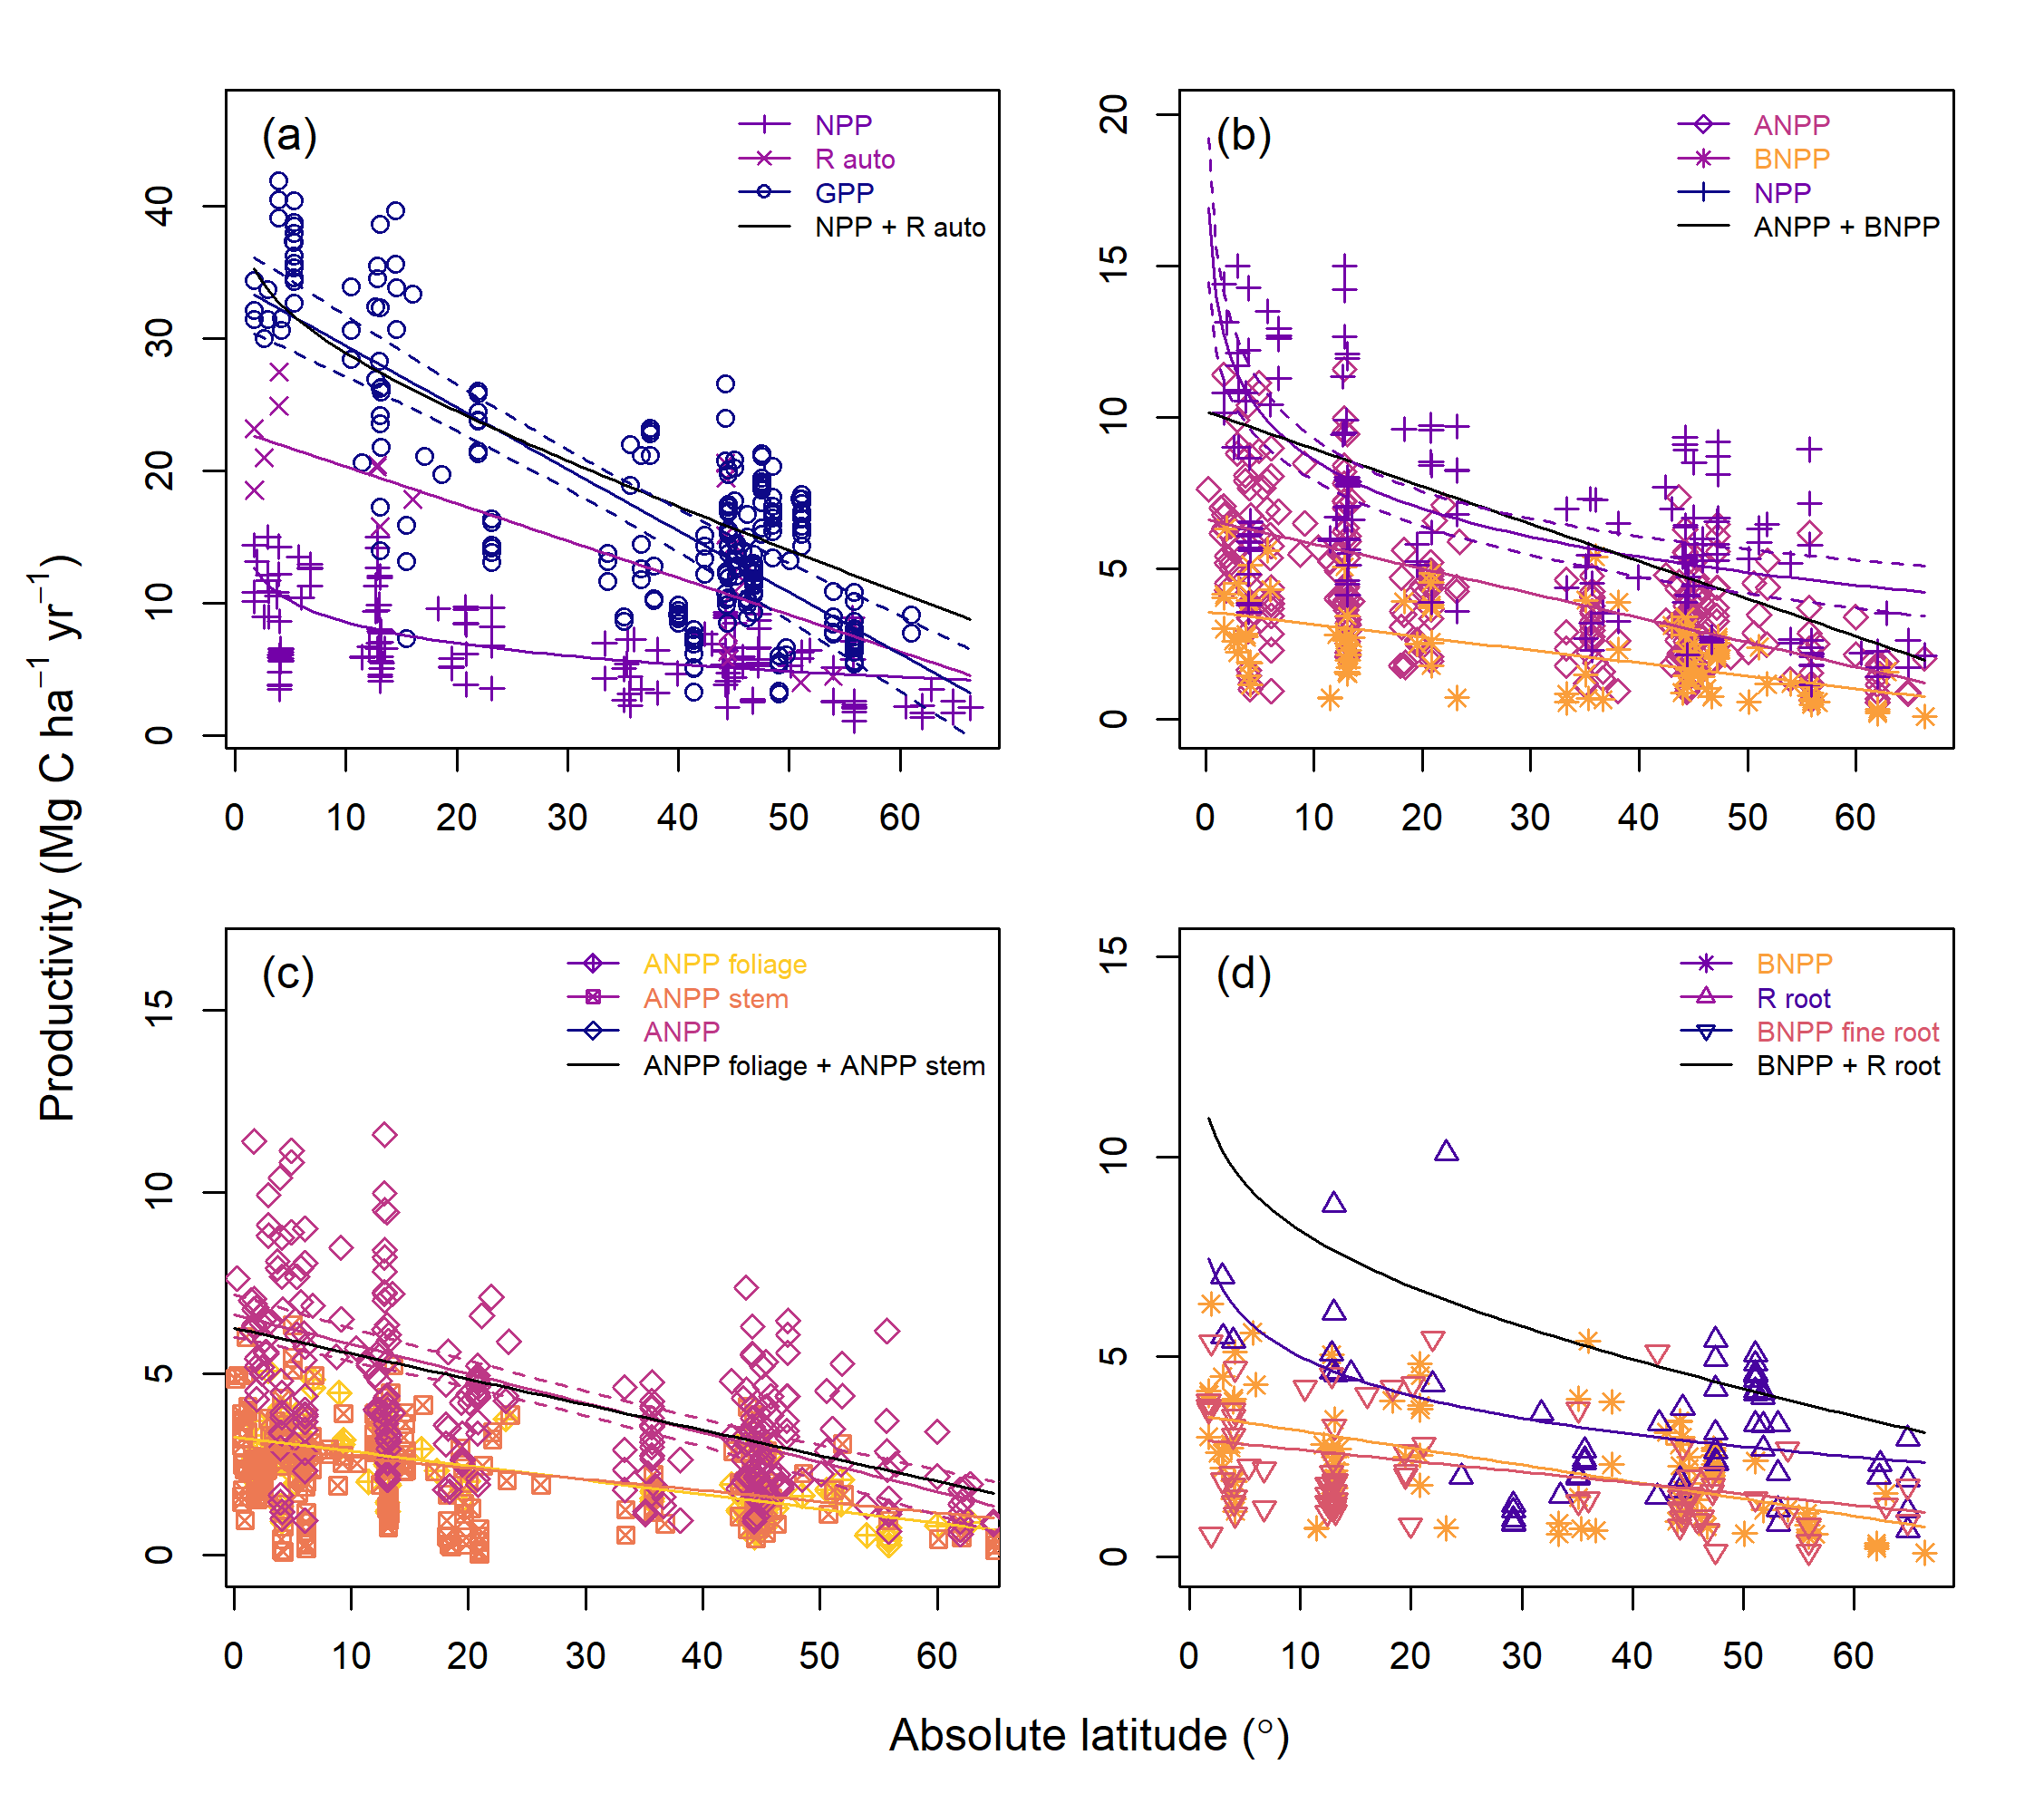
\includegraphics[width=1\linewidth]{combined_stacked} \caption{Latitudinal trends in forest autotropic carbon flux. Lines of best fit are plotted according to the best model selected during analysis. All regressions are significant $(p<0.05)$. Each panel shows major C fluxes together with component fluxes. Also plotted are predicted trends in the major C fluxes based on the sum of component fluxes. 95\% confidence intervals are plotted for the major flux for comparison with predicted trends. In (d),  which shows three belowground fluxes, the major flux, total belowground carbon flux, is one for which we have no data}\label{fig:unnamed-chunk-7}
\end{figure}

In general, smaller component fluxes summed approximately to larger
fluxes across the latitudinal gradient (Fig. 2). That is, modelled
estimates of \(GPP\), generated from the sum of \(NPP\) and
\(R_{auto}\); \(NPP\), generated from the sum of \(ANPP\) and \(BNPP\);
and \(ANPP\), generated from the sum of \(ANPP_{foliage}\) and
\(ANPP_{woody-stem}\), fell completely within the confidence intervals
of the regressions of field estimates of \(GPP\), \(NPP\), and \(ANPP\),
respectively.

We found little evidence that allocation between fluxes varied
substantially with latitude or climate (Fig. S3). Of the 7 FACF ratios
regressed against latitude and three climate variables (MAT, MAP,
temperature seasonality), there were only four signficant relationships,
all with \(R^2 \le 0.2\) (Fig. S3). Specifically, the proportion of NPP
allocated to \(ANPP_{foliage}\) increased weakly with MAT
(\(R^2=0.20\)), and the proportion of \(NPP\) allocated aboveground
(\(ANPP\)) decreased weakly with latitude (\(R^2=0.11\)) and temperature
seasonality (\(R^2=0.17\)), while increasing with MAT (\(R^2=0.11\)).
There were no significant results from regressing ratios of carbon
fluxes against latitude, or against any of the climate variables.

\emph{How do FACF relate to MAT and MAP?}

All FACF increased linearly with MAT, and we found no support for a
saturation point of FACF with MAT (all p\textless{}0.05; Figs. 3-4,
S4-S5, Table S2). As with latitude, MAT tended to explain more variation
in the larger FACF (\(GPP\), \(NPP\), \(ANPP\), \(R_{auto}\)) and
\(ANPP_foliage\) (all \(R^2\)\textgreater{} 0.4) than in subsidiary and
belowground fluxes (\(ANPP_{woody-stem}\), \(R_{root}\),
\(BNPP_{root-fine}\); all \(R^2\)\textless{} 0.25).

MAP was a significant (p\textless{}0.05) predictor of all FACF but
\(ANPP_{woody-stem}\) (Figs. 4a, S4-S5; Table S2). However, it explained
little variation: with the exception of \(R_{auto}\), MAP explained at
most 37\% of variation in FACF. For the majority of FACF, a polynomial
model was the best fit. FACF generally increased with precipitation, up
until a saturation point at between 3000 and 4000mm annual
precipitation, above which they started to decrease (Figs. 4, S4-S5).
The notable exception to this was GPP: the model indicated that GPP
continued to increase with precipitation up to measures of at least
5000mm annually (p\textless{}0.0001, \(R^2\) = 0.33. Data above this
point were not available, but the model trend indicated that the
saturation point for this model would be around 5000mm MAP.

There was a significant additive effect of MAT and MAP on \(GPP\),
\(ANPP\) and \(R_{auto}\) (Fig. 3, Table S3). Accounting for MAT, MAP
had a substantial positive effect on \(GPP\) and \(R_{auto}\) and a
small negative effect on \(ANPP\). There was a significant interactive
effect between MAT and MAP for \(NPP\) and \(ANPP_{woody-stem}\) (Fig.
3, Table S3). The interaction was negative for \(NPP\) and positive for
\(ANPP_{woody-stem}\). For \(ANPP_{foliage}\), \(BNPP\),
\(BNPP_{root-fine}\), and \(R_{auto-root}\), MAP did not have a
signficant effect when accounting for MAT (Fig. 3, Table S3). For the
variables which showed a significant interactive or additive effect
between MAT and MAP, no other climate variable, in combination with MAT,
significantly improved on that model. \{\textbf{need to confirm this
given changes in MAT MAP results (or you could just drop the
sentence.)}\}

\begin{figure}[H]
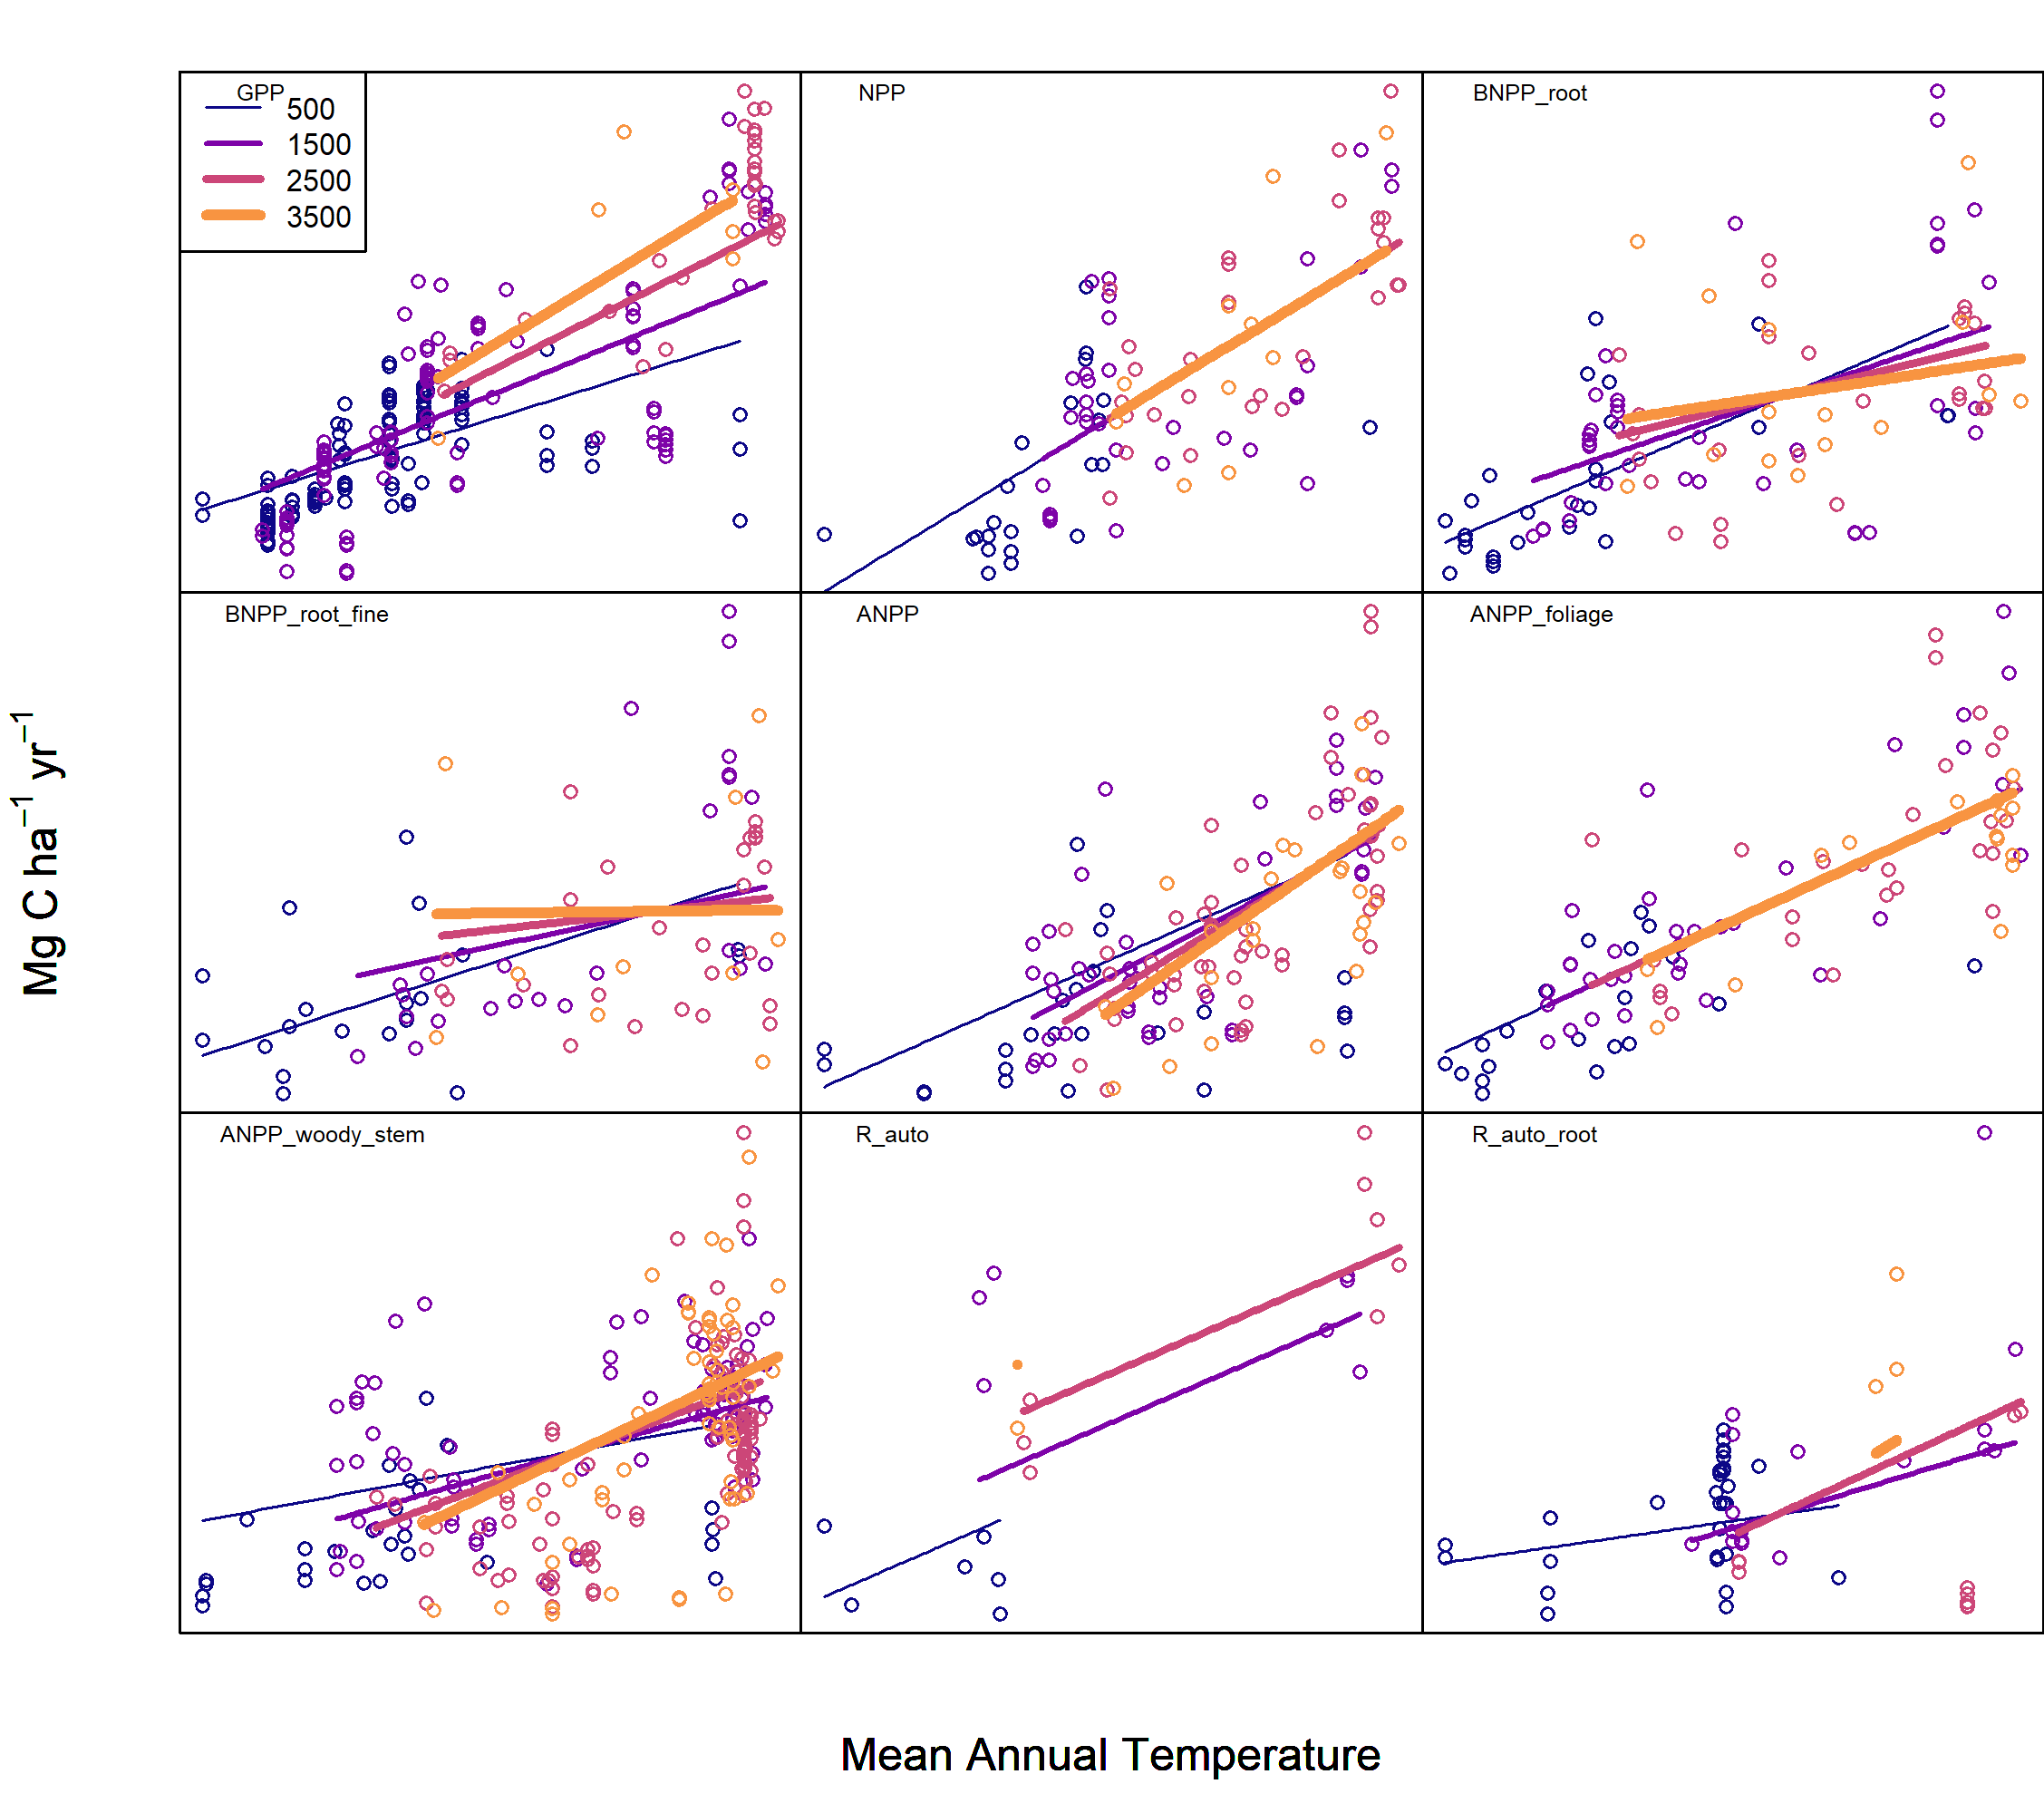
\includegraphics[width=1\linewidth]{mat_map_interaction} \caption{Interactive effects of mean annual temperature and mean annual precipitation on FACF. For visualization purposes, data points are grouped into bins of 0 - 1000, 1001 - 2000, 2001 - 3000, and >3000mm mean annual precipitation, and lines of best fit models are plotted for mean annual precipitation values of 500, 1500, 2500, and 3500mm. All regressions are significant $(p<0.05)$.}\label{fig:unnamed-chunk-8}
\end{figure}

\emph{How do FACF relate to other climate variables?}

Our results indicated that FACF were most strongly explained by
temperature at the global scale, with temperature-related climate
variables coming out as strong predictors of FACF. In addition to MAT,
several of its correlates (Fig. S2) were consistently identified as
strong univariate predictors of FACF: temperature seasonality, annual
temperature range, annual frost days, PET, and length of growing season
(Figs. 4, S4-S7).

We found a significant relationship between C flux and potential
evapotranspiration for all FACF. \(ANPP_{foliage}\),
\(BNPP_{root-fine}\) and \(R_{root}\) increased linearly with PET;
however, all other fluxes showed a polynomial relationship with PET
(Fig. 4c, S4-5; Table S2). We found strong evidence for a saturation
point or peak with PET: FACF tended to increase at values below 1000mm,
before saturating between 1200 and 1700mm. There was also evidence that
FACF begin to decrease at values above 1800mm PET.

Vapour pressure deficit was a significant predictor of C flux for all
FACF. \(BNPP_{root-fine}\) showed a linear relationship with vapour
pressure deficit (\(R^2\) = 0.07, p\textless{}0.05), but all other
fluxes showed a polynomial relationship (Figs. 4d, S4-5; Table S2). FACF
initially increased with vapour pressure deficit, before saturating at
around 0.8 kPa, after wich point they began to decrease.

All fluxes, with the exception of \(R_{root}\), showed a positive linear
relationship with solar radiation (Figs. S4-S5, Table S2). Solar
radiation explained a low proportion of variability in all FACF,
explaining less than 20\% of the variation in each flux, with the
exception of\(R_{auto}\) (\(R^2\) = 0.26, p\textless{}0.05).

Annual wet days, cloud cover, and aridity were poor or non-significant
explainers of variation in FACF, explaining less than 20\% of the
variation in each of the carbon fluxes (Figs. S4-S5; Table S2).

\begin{figure}[H]
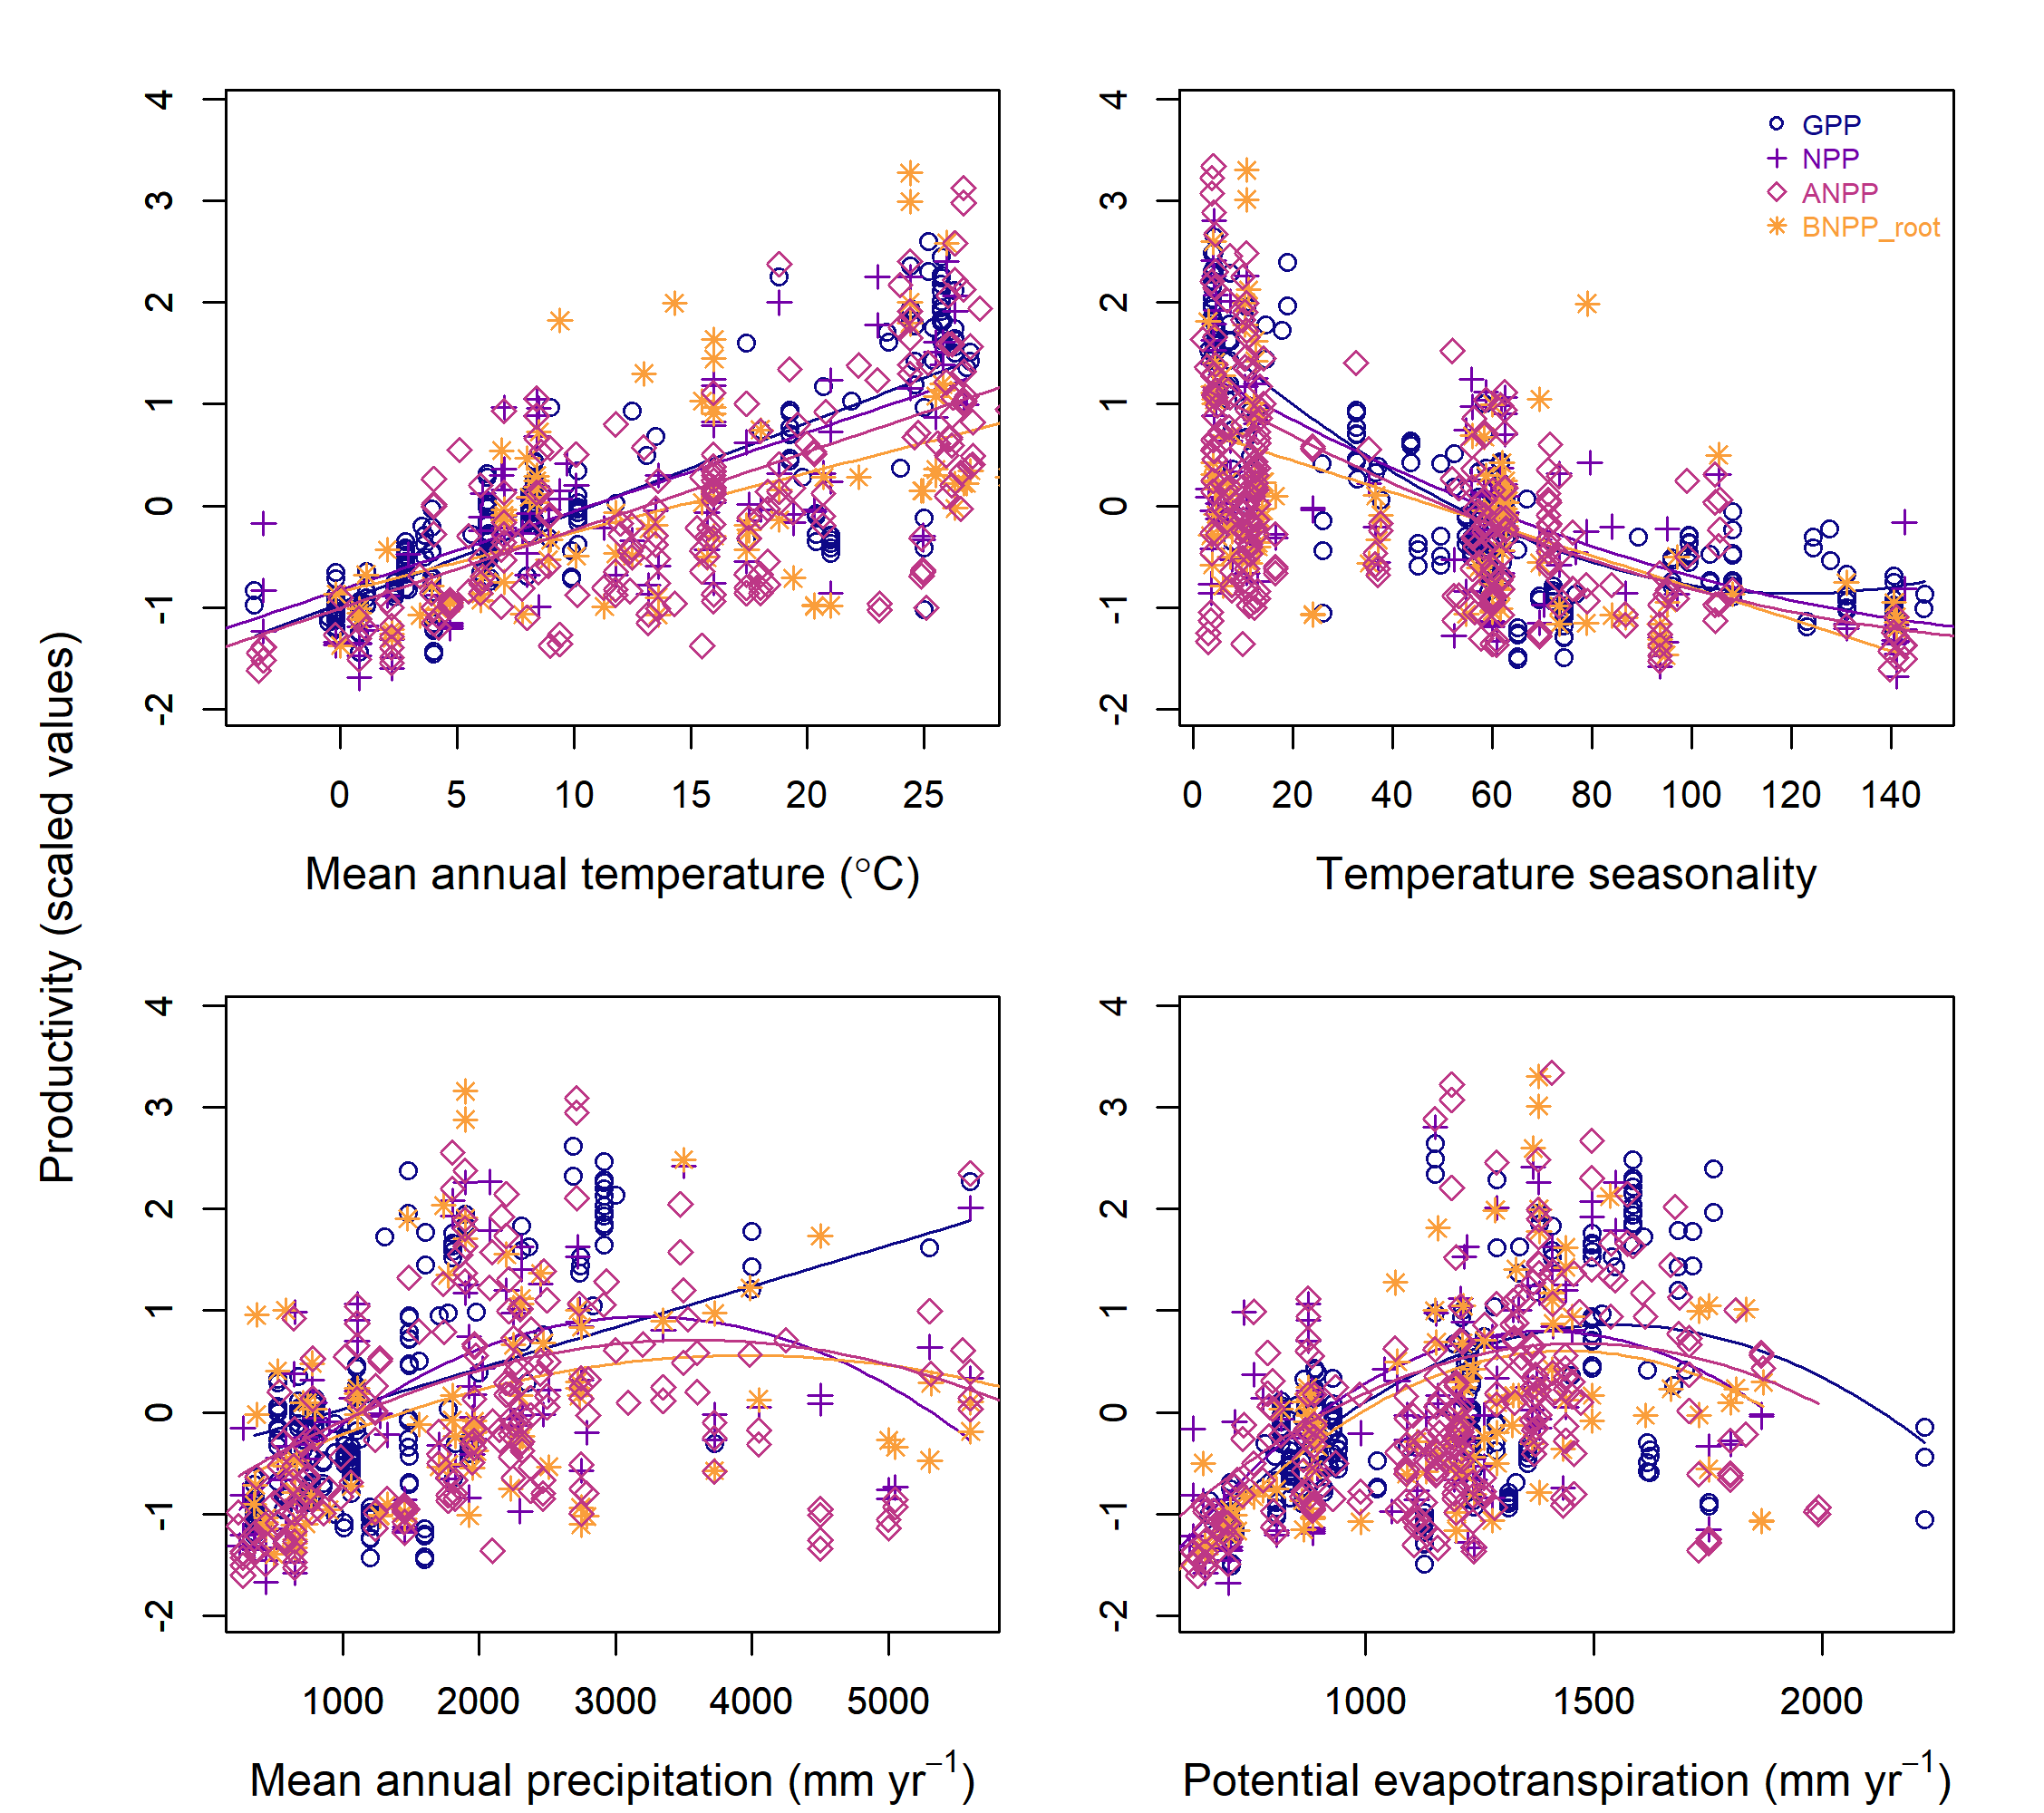
\includegraphics[width=1\linewidth]{combined_plots} \caption{Plots of carbon fluxes against (a) mean annual temperature; (b) mean annual precipitation; (c) potential evapotranspiration, (d) vapour pressure deficit; (e) temperature seasonality; (f) length of growing season. For visualization purposes, data for each flux was rescaled with a mean of 0 and standard deviation of 1. Lines of best fit are plotted according to the best model selected during analysis (**see issue 47**). All regressions are significant $(p<0.05)$.}\label{fig:unnamed-chunk-9}
\end{figure}

\emph{What is the role of seasonality in explaining FACF?}

Temperature seasonality was a significant predictor of FACF. \(GPP\),
\(NPP\), \(ANPP\), and \(R_{root}\) exhibited a polynomial relationship
with seasonality (all p\textless{}0.05; Figs. 4e, S6-7; Table S2).
\(ANPP_{foliage}\), \(ANPP_{woody-stem}\) and \(R_{auto}\) decreased
linearly with temperature seasonality (all p\textless{}0.05; Figs. 4e,
S6-S7; Table S2). Temperature seasonality was strongly correlated with
annual temperature range, which was likewise a similarly strong
predictor of FACF (Table S2).FACF were highest where temperature
seasonality = 0, and at an annual temperature range of 15\(^\circ\)C or
lower.

In contrast, there was no significant effect of precipitation
seasonality on FACF, and both maximum vapour pressure deficit, and water
stress months were poor or non-significant explainers of variation in
FACF (Figs. S6-S7; Table S2).

We found a significant relationship between length of growing season and
FACF, with all fluxes showing a linear increase with length of growing
season (Figs. 4e, S6-S7; Table S2). Length of growing season was a
strong predictor of FACF, explaining 51\% of variation in GPP, 39\% of
variation in NPP, and 34\% of variation in ANPP, but it was a weaker
predictor than MAT for all fluxes analysed (Table S4).

\emph{Within the growing season, how do FACF vary with climate?}

When FACF were standardized by growing season length, correlations with
growing season climate--including temperature, precipitation, solar
radiation, and PET--were generally weak (Figs. S8-S9). Speficifally,
\(ANPP\) increased with growing season temperature (\(R^2\) = 0.10,
p\textless{}0.001) and precipitation (\(R^2\) = 0.04, p\textless{}0.05).
Similaryly, \(ANPP_{foliage}\) increased slightly with growing season
temperature (\(R^2\) = 0.16, p\textless{}0.01) and precipitation
(\(R^2\) = 0.09, p\textless{}0.05). Growing season solar radiation had a
positive influence on \(GPP\) (\(R^2\) = 0.21, p\textless{}0.001),
\(NPP\) (\(R^2\) = 0.21, p\textless{}0.001), \(BNPP\) (\(R^2\) = 0.16,
p\textless{}0.001) and \(BNPP_{fine.root}\) (\(R^2\) = 0.12,
p\textless{}0.01). Growing season PET had a positive influence on
\(GPP\) (\(R^2\) = 0.15, p\textless{}0.01), \(NPP\) (\(R^2\) = 0.18,
p\textless{}0.01), \(BNPP\) (\(R^2\) = 0.23, p\textless{}0.0001),
\(BNPP_{fine.root}\) (\(R^2\) = 0.11, p\textless{}0.05), and
\(ANPP_{woody-stem}\) (\(R^2\) = 0.06, p\textless{}0.05).
\{\textbf{Becky, please verify/ edit the following:} There were no other
signifcant correlations between growing season length-standardized FACF
(9 variables in Table 2) and growing season climate (\textbf{which
variables?})\}.

\subsubsection{Discussion}\label{discussion}

Our analysis of a large global database (ForC) reveals how autotrophic
carbon fluxes in mature forests vary with latitude and climate on a
global scale. We show that, across all nine FACF analyzed, C cycling
decreases continually with latitude (\emph{H1.1}; Fig. 2)--a finding
that confirms multiple previous studies but contradicts the idea that
productivity of temperate forests rivals that of tropical forests
\citep{huston_global_2009}. The FACF generally increase in proportion to
one another (\emph{H1.2}), with few differences in allocation detectable
at this global scale (Fig. S2) and with component fluxes summing
appropriately to larger fluxes (Fig. 2), indicating no major, systematic
omissions or overestimations of flux components. However, climate
explained lower proportions of variability among subsidiary C fluxes
(\emph{e.g.}, \(ANPP_{woody}\), \(BNPP_{fine.root}\), \(R_{auto-root}\);
Fig. 2; Table S2). Latitudianal variation in FACF is primarily
attributable to temperature-related variables (\emph{H3, H4}),
particularly MAT (Figs. 3-4). Water availability is also influential,
but generally of secondary importance across the range represented in
our database (Figs. 3-4). Temperature seasonality and growing season
length are closely correlated with MAT and are strong predictors of FACF
(\emph{H4}; Figs. 4e-f, S2, S6-S7), though growing season length doesn't
improve upon MAT as a predictor. Within the growing season, the
influence of climate on C cycling is smaller but still significant for a
number of FACF (\emph{H5}; Fig. S9; Table S4). These findings clarify
the big picture of how FACF vary with latitude and climate on a global
scale.

Past studies have differed in their conclusions regarding the
relationship between FACF and latitude or its correlates (Table 1,
\emph{H1}; \textbf{REFS})--quite possibly because of lack of
standardization with respect to stand age and disturbance history. Our
findings indicate that, among mature, undisturbed stands, FACF are
unambiguously highest in the tropical regions, and the relationship is
approximately linear (Fig. 2). This contrasts with the suggestion that
productivity of temperate forests is similar to that of tropical forests
\citep{huston_global_2009}. Compared to tropical forests, the temperate
forest biome has experienced more widespread anthropogenic disturbance
and has a larger fraction of secondary stands
\citep{potapov_mapping_2008, poulter_global_2018}, so analyses comparing
across latitudinal gradients without controlling for stand age risk
confounding age with biome effects. In addition, because C allocation
varies with stand age \citep{delucia_forest_2007} (\textbf{See Nobby's
comment in manuscript-draft\_NK.pdf}), age differences may introduce
systematic biases into analyses of FACF across latitude or global
climatic gradients. For example, woody productivity tends to be higher
in rapidly aggrading secondary stands than in old-growth forests, where
proportionally more C is allocated to respiration
\citep{kunert_understanding_2019}. {[}\emph{purpose for respiration/
other compenents} (\textbf{See Nobby's comment in
manuscript-draft\_NK.pdf}){]}.

\textbf{This paragraph needs work--including re-assessment of results,
interpretation, writing} We show that FACF are broadly consistent in
their responses to climate drivers on the global scale (with the
exception of some differences in MAT-MAP interactions; Fig. 3), with no
pronounced trends in C allocation among the variable pairs tested (Figs.
2, S3). Although variation in allocation has been observed along
gradients of elevation \citep{moser_elevation_2011} and water
availability \citep{newman_above-_2006}--along with non-climatic axes of
stand age \citep{litton_carbon_2007}, nutrient availability
\citep{litton_carbon_2007, gill_belowground_2016}, and forest structure
\citep{taylor_greater_2019}--little variation in relation to climate is
apparent at the global scale within ForC, which contains the bulk of
relevant data. Our conclusion, then, is that hypothesized gradients in
allocation along global climate gradients cannot currently be supported
for mature forests, although data quantity and standardization is
currently insufficent to rule out the possibility that such trends
exist. \textbf{bbl: remove following sentence?} Of particular interest
and significance are the relationships amongst \(GPP\), net primary
productivity (\(NPP\) and its components, particularly
\(ANPP_{woody-stem}\)), and respiration (\(R_{auto}\) and components).
There have been suggestions that tropical forests tend to have low
carbon use efficiency (\(CUE\)=
\(NPP\)/\(GPP\)=(\(GPP\)-\(R_{auto}\)/\(GPP\)), which are based on
observations of low \(CUE\) in old-growth tropical forests relative to
(mostly younger) extratropical forests
\citep{delucia_forest_2007, malhi_productivity_2012, anderson-teixeira_carbon_2016},
but our analysis suggests that these low values might more appropriately
be attributed to the fact that these forests are old than to their
tropical climate. Indeed, \(CUE\) is known to decline with forest age
\citep{delucia_forest_2007, collalti_is_2019}, but appears to be roughly
independent of \(GPP\) \citep{litton_carbon_2007}. Among our sites with
relevant data, there is indication that CUE or
\(ANPP_{woody-stem}\)/\(GPP\) increase with latitude (Fig. S3).
Additional measurements with careful methodological standardization
across a consistent set of mature forest sites will be necessary to
determine whether any climate-driven gradients in allocation exist at
the global scale.

One interesting observation was that climate tends to explain more
variation in the major fluxes (\(GPP\), \(NPP\), \(R_{auto}\) - latitude
\(R^2\ge\) 48\%) than in subsidiary fluxes (latitude \(R^2\)
\textless{}27\% for \(BNPP_{fine.root}\),
\(R_{auto-root}\),\(ANPP_{woody-stem}\)) (Fig. 2; Table S2). There are
two, non-exclusive, potential explanations for this. First, it may be
that methodological variation is larger relative to flux magnitude for
some of the subsidiary fluxes. Belowground fluxes in particular are
difficult to quantify, and measurement methods for the belowground
fluxes considered here may be measured through fundamentally different
approaches (\emph{e.g.}, minirhizotrons, ingrowth cores, or sequential
coring for \(BNPP_{root-fine}\); root exclusion, stable isotope
tracking, or gas exchange of excised roots for \(R_{auto-root}\)), and
sampling depth is variable and often insufficient to capture the full
soil profile. \(ANPP_{woody-stem}\), which is also poorly explained by
latitude or climate, is more straightforward to measure but is subject
to variability introduced by differences such as biomass allometries
applied and minimum plant size sampled (\textbf{bbl: cite
e.g.~Huntzinger?}). However, methodological variation and uncertainty
affect all of fluxes considered here--not necessarily any less than the
aforementioned, and some of the larger fluxes that vary more strongly
with respect to climate (\(ANPP\), \(NPP\)) are estimated by summing
uncertain component fluxes. Second, differences among variables in the
proportion of variation explained by climate may be attributable to more
dicrect climatic control over \(GPP\) than subsidiary fluxes. That is,
subsidiary fluxes may be shaped by climate both indirectly through its
influence on \(GPP\) and respiration and directly through any climatic
influence on C allocation, as well as many other local- and
regional-scale factors (\textbf{REFS}).

The latitudinal gradient in FACF (Fig. 2) is driven primarily by
temperature-related climate variables, and secondarily by moisture
availability (Table 1, \emph{H2-H3}; Figs. 3-4). Because many climate
variables co-vary across the latitudinal gradient (Fig. S2), because
climatic drivers affect forest carbon flux on much shorter time scales
than can be captured by annual climate summary variables, and because
both climatic conditions and C flux vary intra- and inter-annually
around the long-term means, it is not appropriate to attempt to identify
any one mean annual climate variable as a mechanistic driver of FACF.
However, it remains informative to consider these relationships. We find
that temperature-related climate variables (\(MAT\), temperature
seasonality, \ldots{}\textbf{LIST}) explain the highest proportion of
variability in FACF, and among these, \(MAT\) is generally the best
predictor--perhaps because site-specific MAT is recorded for the
majority of sites in ForC, whereas other variables are extracted from
global gridded data products (Table S1). The effects of temperature are
modified by moisture availability, with reduced FACF under hot and dry
conditions (\emph{i.e.}, high PET, high deficit; Fig. 4c-d) and
sometimes under very high precipitaiton (Figs. 3, 4b). Negative effects
of very high precipitation on FACF have been observed previously
(\textbf{REFS}) and are attributable to nutrient and light limitations
(\textbf{REFS}). Thus, although temperature and water availability
jointly and interactively drive global-scale patterns of FACF.

FACF are negatively correlated with temperature seasonality (Table 1,
\emph{H4}; Fig. 4e), and is minimal during cold- or dry- dormant
seasons. To account for this, a number of analyses seeking to
characterize global-scale effects of climate on productivity have
examined the relationship of C flux per month of the growing season with
growing season climatic conditions (Table 1, \emph{H5}; \textbf{REFS}).
We found that the sort of simple metric needed to define growing season
at a global scale was uncertain for temperature and problematic for
moisture (\textbf{WORK ON THIS}). A temperature-defined growing season
length had stong positive correlation with FACF (Fig. 4f), but explained
less variation than \(MAT\). Dividing FACFs by growing season length to
yield FACF per growing season month removed the majority of
climate-related variation, supporting the idea that the latitudinal
gradient in FACF is attributable more to shorter growing seasons at high
latitudes than to inherently lower rates of photosyntheiss or
respiration by high-latitude forests (\emph{{[} Enquist et al. 2007 GCB-
but check{]}}). However, there remained a number of significant
correlations with growing season climatic conditions, suggesting that
climatic conditions remain influential within the growing season. We
conclude that while correcting for growing season length takes analyses
a step closer to mechanistic linkage of instantaneous C flux rates to
environmental conditions, it remains very crude relative to the the
timescales on which climate affects plant metabolism and does not
advance statistical predictive power. Rather, mechanistic accounting for
climatic effects on global FACF patterns requires models representing
physiologically meaningful timescales (\emph{e.g.}, \textbf{refs}).

Our analysis clarifies how FACF vary with latitude and climate on a
global scale, with some important implications for how forest carbon
cycling relates to climate and, by extension, how it is likely to
respond to climatic warming. Our findings show that higher temperatures
with similar moisture availability result in a generalized acceleration
of FACF (Figs. 2-3). This is consistent with observations of
continental- to global-scale increases in \(GPP\)
\citep{li_mapping_2019} and \(ANPP_{woody stem}\)
\citep{brienen_long-term_2015, hubau_asynchronous_2020}, along with some
C cycle components not considered here--tree mortality
\citep{brienen_long-term_2015, mcdowell_drivers_2018}, soil respiration
\citep{bond-lamberty_global_2010}, and heterotrophic soil respiration
\citep{bond-lamberty_globally_2018}. However, increasing C flux rates
are not universal \citep{rutishauser_testing_2020} (\textbf{MORE REFS}).
This is likely because factors other than rising temperatures are at
play, including changes to other aspects of cliamte, atmospheric
pollution (CO\textsubscript{2}, SO\textsubscript{2},
NO\textsubscript{x}), and local disturbances. Morevoer, forest ecosystem
responses to climatic changes outside the temperature range to which
forest communities are adapated and acclimatized will not necessarily
parallel responses across across geographic gradients in climate.
Nevertheless, as we enter a period of accelerating climatic change,
understanding of the fundamental climatic controls on FACF sets a
foundation for understanding patterns of change.

\subsection{misc content for
discussion}\label{misc-content-for-discussion}

\begin{itemize}
\item
  the observed positive interaction between MAT and MAP for
  \(ANPP_woody\) is consitent with the \citet{taylor_temperature_2017}
  analysis showing such an interaction for \(ANPP\) in tropical forests.
  Similar to their analysis, we find a cross-over point at
  \textasciitilde{}20C. However, we don't find such an interaction for
  \(ANPP\), and we show a contrasting negative interaction for \(NPP\).
  Some of this is may be stochasitic/ driven by composition of the
  dataset, and the interactions we observe are not internally
  consistent.
\item
  consistent with \citep{hofhansl_new_2015} (\textbf{verify}) , we found
  a slight tendency for warmer sites to have higher aboveground
  allocation
\end{itemize}

-results are consistent with \emph{Muller-Landau et al., in review}

\subsubsection{Acknowledgements}\label{acknowledgements}

Scholarly Studies ForestGEO Compilation of the ForC database was
originally funded by DOE

\bibliography{library.bib,packages.bib}


\end{document}
